\begin{figure}[htb!] 
\centering
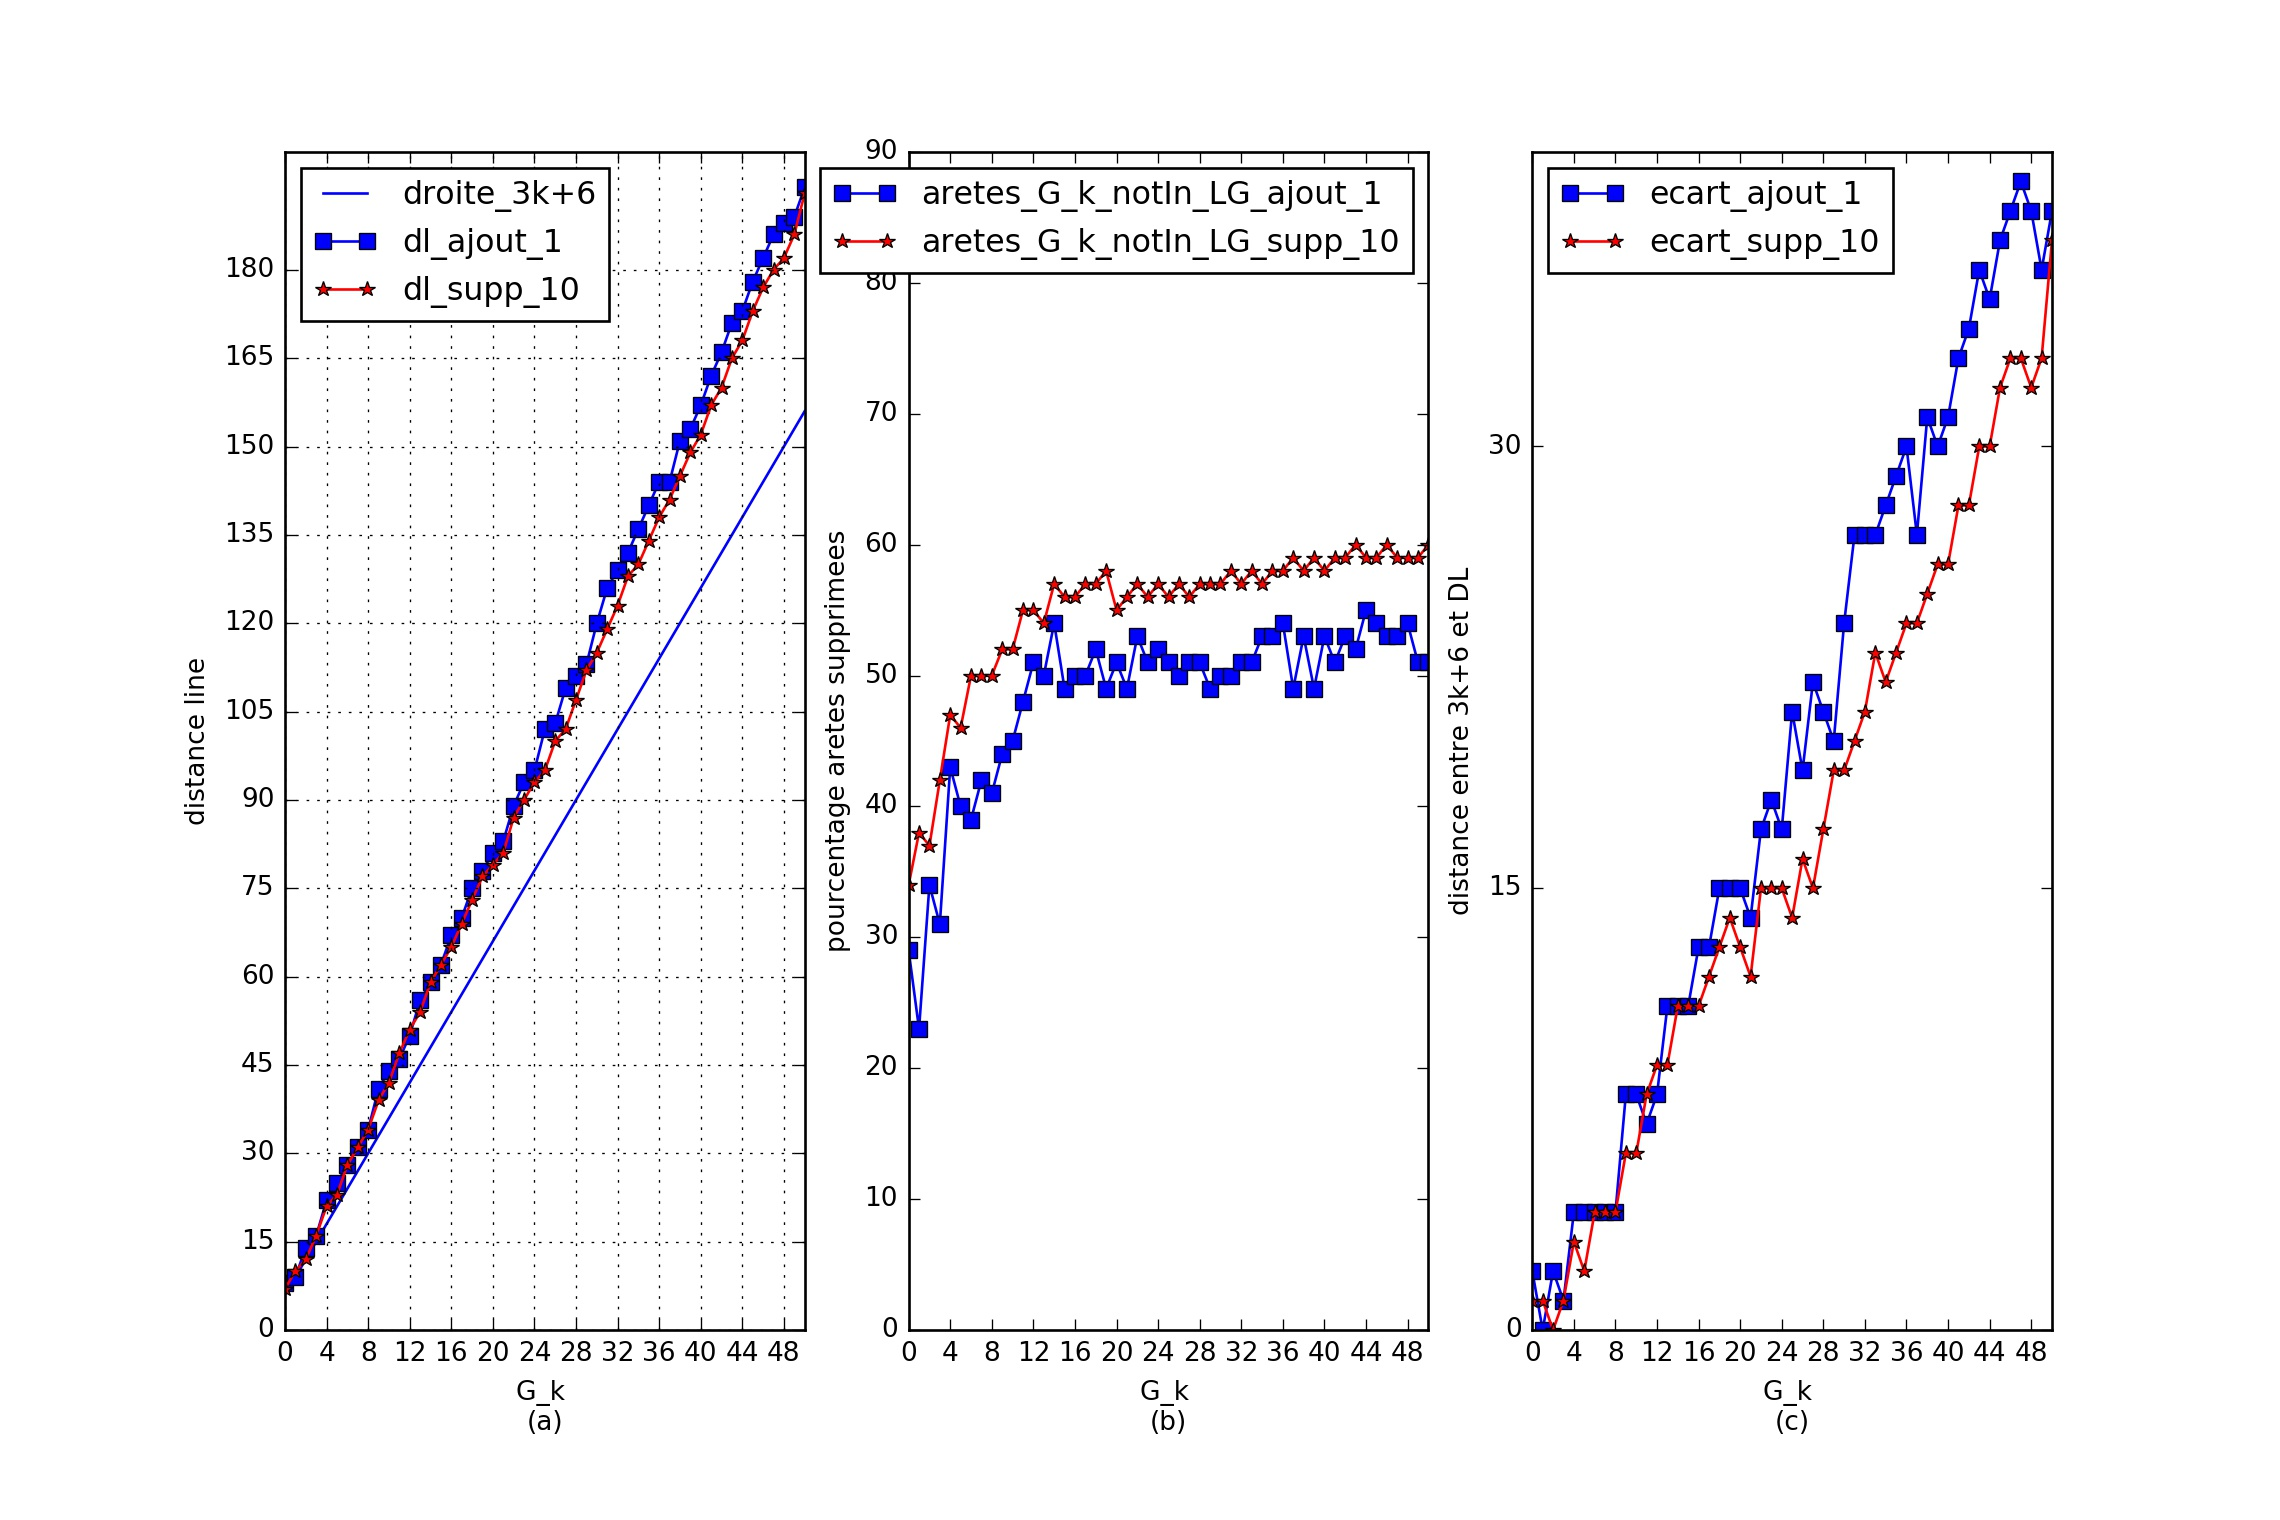
\includegraphics[scale=0.250]{comparaison_prior_ajout_wi_1_supp_wi_10_distance_line_vs_3k_6_graphe_iourte.jpeg}
\caption{  (a) fonction de co\^ut {\em suppression} : la courbe {\em dl\_ajout\_1} d\'esigne la correction par la priorisation des ar\^etes ajout\'ees avec un poids $\phi^{+} = 1$  pour une ar\^ete ajout\'ee et un poids $\phi^{-} = 1$  pour une ar\^ete supprim\'ee.
 La courbe {\em dl\_supp\_10} d\'esigne la correction par la priorisation des ar\^etes supprim\'ees avec un poids $\phi^{-} = 1$  pour une ar\^ete supprim\'ee et un poids $\phi^{+} = 10$  pour une ar\^ete ajout\'ee,
 (b) taux de suppression d'ar\^etes dans  $G_0^k$ pour les priorisations  {\em dl\_ajout\_1} et  {\em dl\_supp\_10},
 (c) la diff\'erence de distances line entre les priorisations {\em dl\_ajout\_1} et  {\em dl\_supp\_10}  et la droite $y=3k+6$. }
\label{priorAjout1Supp10} 
\end{figure}

\'Etant donn\'ee que la fonction de co\^ut {\em ajout} produit de moins bons r\'esultats, nous allons comparer les fonctions {\em suppression} et {\em unitaire}. La courbe {\em dl\_supp\_1} d\'esigne la fonction {\em suppression}. Dans cette fonction, nous attribuons un poids $\phi^{-} = 1$ pour la suppression d'ar\^etes et un poids $\phi^{+} = 10$ pour l'ajout d'ar\^etes.
\newline
Dans la figure  \ref{priorAjout1Supp10}(a), les courbes {\em dl\_ajout\_1} et {\em dl\_supp\_10} sont confondues \`a la profondeur $k \le 20$ et au d\'el\`a de $k > 20$, il existe un leger \'ecart entre ces deux courbes. 
Cet \'ecart est caus\'e par la suppression d'ar\^etes dans la fonction {\em suppression}. 
En effet, la courbe {\em aretes\_G\_k\_notIn\_LG\_supp\_10} qui correspond \`a la fonction {\em suppression} est monotone pour $k \ge 20$ parce que le nombre d'ar\^etes supprim\'ees est quasi constant m\^eme si ce nombre est \'elev\'e (voir figure \ref{priorAjout1Supp10}(b)). L'algorithme ajoute peu d'ar\^etes pour trouver un line-graphe connexe. Cela engendre que cette courbe {\em dl\_supp\_10} est en dessous de celle de {\em dl\_ajout\_1} et elle se rapproche de la droite $y = 3k +6$. 
Pour la courbe {\em aretes\_G\_k\_notIn\_LG\_ajout\_1} associ\'ee \`a la fonction {\em ajout}, le nombre d'ar\^etes varie entre $49\%$ et $51\%$ pour $k \ge 20$ (voir figure \ref{priorAjout1Supp10}(b)). Cette variation engendre des baisses de distances line lorsque les pourcentages d'ar\^etes supprim\'ees sont \`a leurs extremums (cas de $G_0^{28}$ et  $G_0^{36}$).
\newline
Nous pouvons conclure que la fonction {\em suppression} donne de meilleurs r\'esultats que celle {\em unitaire} quand la profondeur augmente $k \le 20$. En dessous de cette valeur $k < 20$, les fonctions de co\^uts n'ont aucune influence sur les distances line calcul\'ees.




%au terme de nos simulations nous retenons que la phase de correction produit de bons resultats en presence de fausses negatives plus nombreux que des fausses positives.